\section{Methodology and Approach}
To assess the feasibility of this approach and test user's empathy with the pre-made metahumans a controlled experiment will test whether the virtual avatars are able to convey the same emotional depth and realism as a real person (RQ1).

To do so, participants will be exposed to one of the following pre-recorded content: a) a male person, b) a male metahuman, c) a female person, d) a female metahuman, all of which will feature the same narrative (see Appendix A). The metahumans were created to match the appearance of the real person (Figure 9) as close as possible while keeping performance levels high (by using only optimized assets). This was done in order to avoid introducing excessive third-variable bias \cite{ROT19}, and the story was chosen from a specific subreddit (i.e., an online community where people ask others for advice) based on the amount of upvotes (1500) and number of comments (304) received on Reddit, as it provides a metric on user engagement and, therefore, we believe will help elicit empathy in the participants.


\begin{figure}[h!]
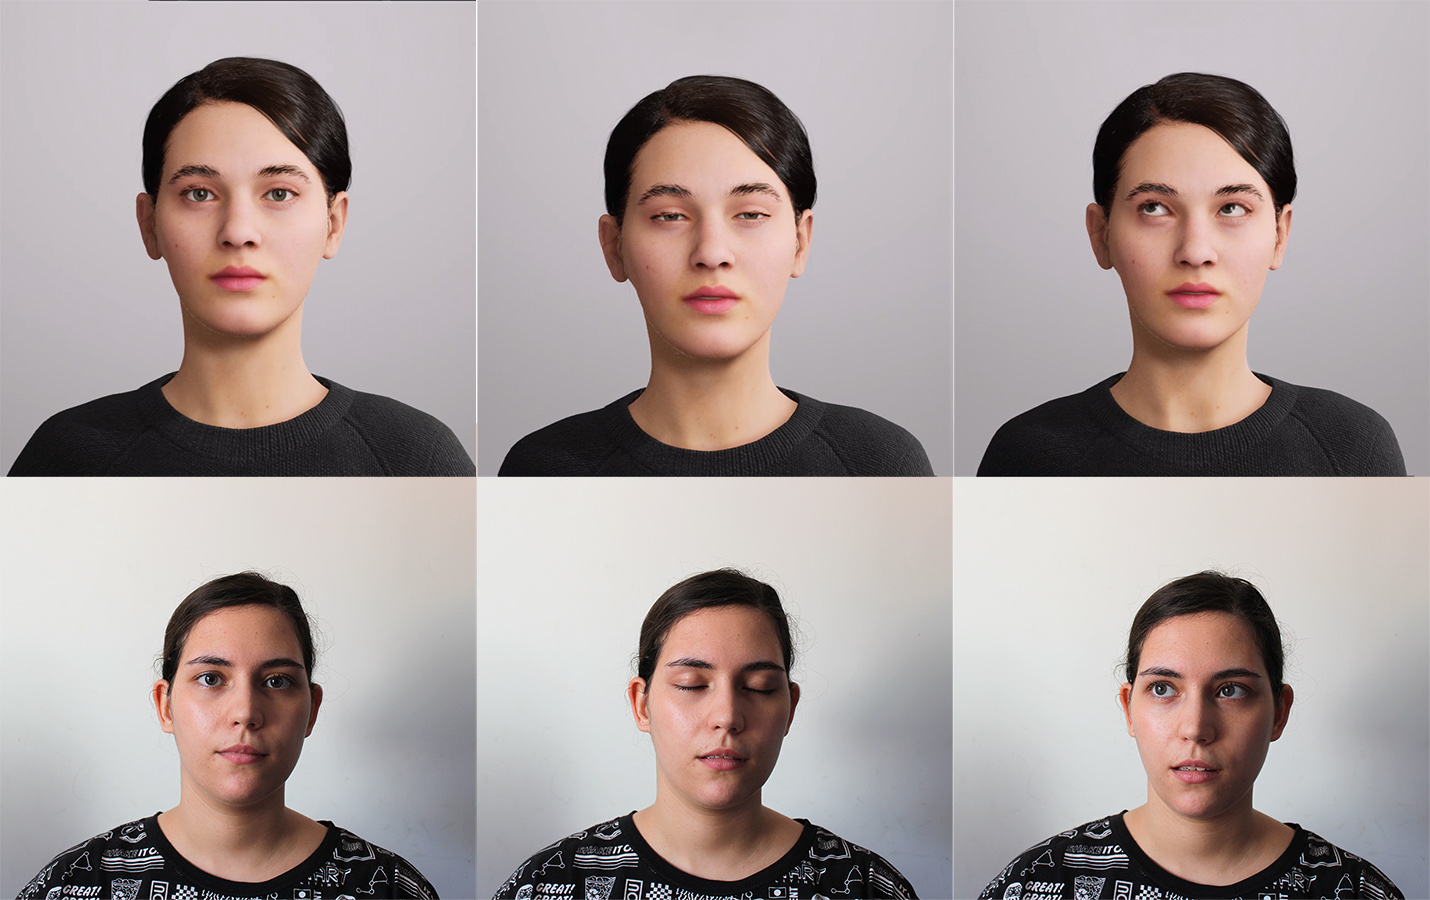
\includegraphics[width=0.48\textwidth]{figures/personavatar.jpg}
\centering
\caption{Different expressions in both the custom metahuman and the actor}
\end{figure}

As it was not necessary to use the developed prototype in its entirety for this study, only the communication between the apple device and the Unreal Engine 4 for the metahuman's animation is required. As a result, the use of customized avatars has no effect on performance levels since all that is required to conduct this experiment is the capture of a local video from the UE4 application. These issues do not occur in local tests.

To avoid revealing the experiment's true purpose, and thus distorting the results, participants will be asked to answer some general questions about themselves (from the Big Five Inventory) in addition to the Toronto Empathy Questionnaire \cite{SPR03}, and the questionnaire developed to measure participants' empathy levels, as proposed by \cite{ROT19, ZIB19}. 
The experiment was accepted by the university's Data Protection Officer and authorized by the Ethics Committee and participants will be recruited via email, sent to the general undergraduate student population from Madeira University, where they will be briefed about the study's broad, general topic.
The ones who agree to participate in the test will be asked to complete basic demographic questions and a personality questionnaire used to measure their baseline empathy levels prior to the video stimuli, and each participant will be randomly redirected to one of the pre-recorded video contents using \cite{FER19} and later asked some follow-up questions.

\subsection{Evaluation}
On the pre-test (Appendix B), the Toronto Empathy Questionnaire \cite{SPR03} will be utilized as a control variable, consisting of 16 items (e.g., "I become irritated when someone cries", 1=strongly disagree, to 5=strongly agree). To dispel any suspicions regarding the study's genuine goal, five items from the Big Five Inventory \cite{JOH91} will be incorporated into the questionnaire.

The dependent measures' questions will then be answered on a seven-point Likert-type scale (1=totally disagree, 7=totally agree) on the post-test (see Appendix C), based on the work of Bailenson et al. \cite{BAI03}.

We will use four questions to assess the video's perceived authenticity and social presence, presenting the statements ("I feel that the person is watching me and is aware of my presence", "The thought that the person is not a real person crosses my mind often", "The person appears to be conscious and alive to me", "I perceive the person as being only a computerized image, not as a real person") with the above-noted Likert-type scale.

Then, empathy will be tested using items adapted from the Interpersonal Reactivity Index \cite{DAV83} that deal with cognitive and affective empathy. Three items will be used to test cognitive empathy: "I understand what made her get upset", "Her reactions to the situation are understandable", and “I understand her point of view”. Afterwards three items will be used to measure emotional empathy ("I can relate to her problem", "When I see someone in an unfair situation, I feel frustrated", and “I feel that her emotions are genuine”).

Finally, participants should describe what made them empathize with and/or relate to the person in the video, as well as what they didn't like.

\subsection{Hypothesis}